
Data extraction from various blockchains is a hot topic and there are different projects that have tried to address this problem. A lot of work has been done by business projects, whose source code and methodology is not publicly available. There are also some open source or academic attempts that I will use as a comparison with my work. 

\noindent In the next sections I'll list the most relevant works I found.

\section{Etherscan}

Etherscan \footnote{https://etherscan.io/} is the reference point for accessing data about the Ethereum blockchain. It’s the main explorer that lets people browse historical data trough a web interface. Here users can easily explore transactions, internal calls, token transfers and everything else related to the Ethereum protocol. It’s useful for inspecting singular operations, but it can’t be used for large scale analysis.

One of the most important service they offer is the verification of smart contracts, they host 461,261\footnote{This data was calculated using the CSV file exported from https://etherscan.io/chart/verified-contracts} source codes (as of 17 May 2023) that have been verified to match exactly the deployed bytecode on the  Ethereum chain. 

The process of verification consists in providing Etherscan the exact source code of a Smart Contract, the version of the compiler used, the license selected and the contract address to verify. With this information, Etherscan will try to compile the given data and check if the resulting bytecode equals the one deployed on the blockchain. There are plugins for the most used development tools like Remix or Hardhat that ease this process of verification.

This data is extremely helpful for understanding the semantic of the code deployed, since it's very hard to get useful insights by just looking at the raw bytecode. Many studies are based on these verified contracts.

Etherscan has evolved from being just an Ethereum explorer. They used the huge amount of information indexed to create API endpoints and offer these data to users for a fee. These API endpoints include the standard Ethereum JSON-RPC interface and many more advanced methods, like tokens logic or specific index not supported by the standard RPC. 

On top of that, they also provide live and interactive charts\footnote{Available at https://etherscan.io/charts} about historical Ethereum data.

The same company that is behind the Ethereum Etherscan explorer applied the same logic and technology on other EVM compatible chains, like Polygon\footnote{https://polygonscan.com/} or BNB Smart Chain\footnote{https://bscscan.com/}.

It's important to note that, although they provide almost all the possible available Ethereum data, they haven't shared technical details about how this data is extracted or how it is indexed, users need to trust the company. Another problem is that using their data via the API for large scale analysis is unfeasible since it would be too expensive.


\section{The Graph}

The Graph\footnote{https://thegraph.com/} is a decentralized indexing protocol for blockchain data. It allows users to get structured on-chain data from other users via a GraphQL\footnote{GraphQL is an open source query language created by Facebook.} interface. 

All the data is organized is so called "subgraphs" that are independent data collections that index a small subset of a blockchain network. A common pattern is that a subgraph indexes data from one or a set of few smart contracts all part of a common protocol, like Uniswap. All the available subgraphs can be found on the explorer\footnote{https://thegraph.com/explorer}.

The underlying protocol is composed of multiple actors:

\begin{itemize}
  \item Developers: people with technical knowledge that develop the needed code for creating and maintaining the indices. As of now, the most important pieces of code needed are the mappings from Ethereum events to the stored data (written in AssemblyScript\footnote{https://www.assemblyscript.org/}, a Typescript-like language that is compiled to WebAssembly) and the subgraph manifest, a structured description of all the parts needed by the subgraph in YAML format.  
  \item Indexers: they are responsible for operating a node, this implies indexing the data following a subgraph specification and serving queries.
  \item Curators: they are in charge of finding the best subgraphs to be indexed.
  \item Delegators: they secure the network by locking economical value to certain indexers they choose.
\end{itemize}

All of these actors are economically motivated to perform well, this is achieved via a token economy where the GRT is the currency. It is implemented on the Ethereum chain with a standard ERC20 smart contract\footnote{https://etherscan.io/token/0xc944e90c64b2c07662a292be6244bdf05cda44a7}.

In order to index and serve queries, indexers have to stake 100,000 GRT tokens (roughly equal to 12K USD with the current change). These tokens can be slashed in case the indexer behaves maliciously. The more tokens the indexer stakes and the more queries it can serve. At the same time, indexers are rewarded with GRT tokens in two ways: query fees and annual rewards based on queries served.

According to the specification of the subgraph file\footnote{https://github.com/graphprotocol/graph-node/blob/master/docs/subgraph-manifest.md\#15-data-source}, the only allowed source of data are Ethereum contracts and mappings are restricted to Events. Image 3.2.1, taken from the The Graph official website, shows the flow of data in the protocol. In most cases, this is enough for dApps, since typically all the smart contracts are written in such a way that they emit events when things happen. On the other hand, it is not possible to index all the other kind of information for performing other analysis, such as block data, contract deployments, transactions, contracts destruction, etc. It is also not possible to extract data that was not meant to be extracted, since the emitted events are pieces of information that the developers of the smart contracts explicitly wanted to expose and index. 


\begin{figure}[H]
  \centering
  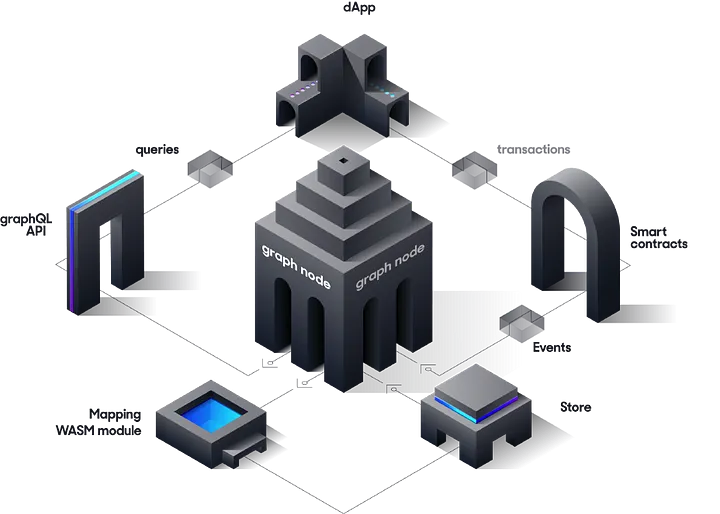
\includegraphics[width=1\textwidth]{Figures/graph-dataflow.png}
  \caption[The Graph data flow]{Data flow of The Graph indexing protocol}
  \label{fig:the-graph-data-flow}
\end{figure}

As of today, the protocol still relies on a central hosted service that uses the subgraphs logic and code to index data, but queries are served from this centralized server for free. This should change in 2023, the network should slowly migrate from this centralized service to the decentralized protocol once the quality of the service will be comparable \footnote{https://thegraph.academy/developers/sunsetting-the-hosted-service/}.

The Graph is the first attempt to decentralize indexing of blockchain data, it's still a project with a lot of work behind the scene. It's the most promising mechanism to make Web3 and dApps more decentralized and less dependant from centralized services. 


\section{Ethereum-ETL}

Lorem ipsum dolor sit amet.

\section{Dune analytics}

Lorem ipsum dolor sit amet.

\section{Xblock-ETH}

Lorem ipsum dolor sit amet.

\section{Web3 providers}

Lorem ipsum dolor sit amet.
